\documentclass[tikz,border=2pt]{standalone}
\usepackage{amsmath,amssymb}
\usepackage{tikz}
\usetikzlibrary{arrows.meta,calc}

\begin{document}
% Cauchy-Schwarz: |x.y| = ||x|| ||y|| |cos theta| <= ||x|| ||y||, because the projection of y
% onto x is never longer than y itself; equality exactly when x and y are parallel.
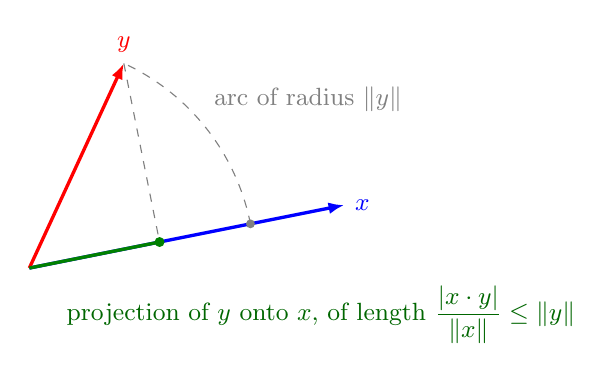
\begin{tikzpicture}[every node/.style={font=\small}, >={Latex[length=2mm]}]
	\coordinate (X) at (4,0.8);
	\coordinate (Y) at (1.2,2.6);
	\coordinate (P) at ($0.4135*(4,0.8)$);
	\draw[gray, dashed] (11.31:2.864) arc (11.31:65.22:2.864);
	\draw[->, blue, very thick] (0,0) -- (X) node[right] {$x$};
	\draw[->, red, very thick] (0,0) -- (Y) node[above] {$y$};
	\draw[dashed, gray] (Y) -- (P);
	\draw[green!50!black, very thick] (0,0) -- (P);
	\fill[green!50!black] (P) circle (1.8pt);
	\fill[gray] (11.31:2.864) circle (1.6pt);
	\node[gray, font=\small, anchor=south west] at (40:2.9) {arc of radius $\|y\|$};
	\node[green!40!black, anchor=north west, font=\small] at (0.35,-0.1) {projection of $y$ onto $x$, of length $\dfrac{|x\cdot y|}{\|x\|}\le\|y\|$};
\end{tikzpicture}
\end{document}
